\section{Thermal Hydraulics}
\label{sec:thermalHydraulics}

\begin{frame}{Material Properties}
  \begin{itemize}
    \item Functional sodium properties from \cite{sodiumProp}.
    \item Clad and sodium thermal conductivity assumed constant \cite{ht9Prop}.
    \item Fuel thermal conductivity assumed a function of temperature
      \cite{fuelProp}.
  \end{itemize}
  \begin{table}
    \caption{Constant Thermal Conductivity for Sodium and HT9.}
    \label{tab:constant_k}
    \begin{center}
      \begin{tabular}{cl}
        \toprule
        Material & $k \units{$\frac{\text{W}}{\text{m K}}$}$ \\
        \midrule
        Sodium &  64.33 \\
        HT9    &  25.81 \\
        \bottomrule
      \end{tabular}
    \end{center}
  \end{table}
\end{frame}

\begin{frame}{Fuel Thermal Conductivity}
  %\begin{align}
  %  \label{eq:kfuel_first}
  %  k_U      &= 21.73 + 1.591 \times 10^{-2} T + 5.907 \times 10^{-6} T^2 \\
  %  k_{Zr}   &= 8.853 + 7.082 \times 10^{-3} T + 2.533 \times 10^{-6} T^2 +
  %    2.992 \times 10^{3} T^{-1} \\
  %  k_{c,Zr} &= -102.0 + 200.1 x_{Zr} - 109.2 x_{Zr}^2 + 
  %    9.435 \times 10^{-3} T + 3.459 \times 10^{-5} T^2 - 0.02093 x_{Zr} \, T \\
  %  \label{eq:kfuel_last}
  %  k_{U-Zr} &= \left( 1 - \sqrt{1-x_{Zr}}\right) k_{Zr} + 
  %    \sqrt{1 - x_{Zr}} \left( \left( 1 - x_{Zr}\right) k_U + x_{Zr} \, k_{c,Zr}
  %    \right) 
  %\end{align}
  \begin{figure}
    \centering
    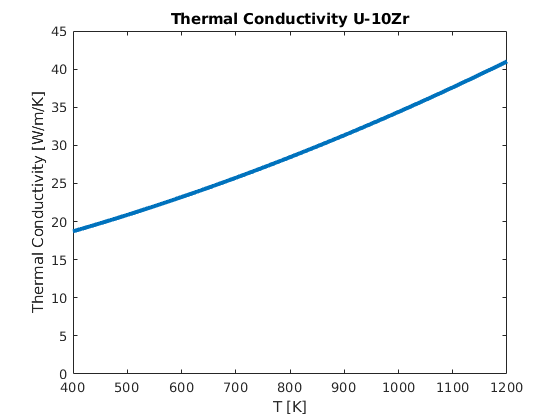
\includegraphics[width=0.7\textwidth]{kfuel_plot}
    %\caption{Variable Thermal Conductivity in Fuel.}
    \label{fig:kfuel_plot}
  \end{figure}
\end{frame}

\begin{frame}{Calculating Reactor Power}
  For a user-input $Q_{Rx}$, a normalization constant is calculated to convert
  unnormalized flux $\widetilde{\phi_{g,e}}$ to normalized flux $\phi_{g,e}$.
  \begin{align}
    \label{eq:normalization_c}
    c &= \frac{Q_{Rx}}{\sum_{g}^{G} \sum_{e}^{N_E} \kappa \Sigma_{f,g,e} \,
      \widetilde{\phi_{g,e}} \, V_e} \\
    \phi_{g,e} &= c \, \widetilde{\phi_{g,e}}
  \end{align}
  Element power is defined.
  \begin{equation}
    \label{eq:elementpwr}
    q_{e} = \sum_g^G \kappa \Sigma_{f,e,g} \, \phi_{g,e} \, V_e .
  \end{equation}
  Assuming all heat generated in the element is generated within the fuel, the
  volumetric heat generation rate is defined.
  \begin{equation}
    \label{eq:elementqppp_fuel}
    q'''_{e} = \frac{q_e}{V_{fuel,e}}
  \end{equation}
\end{frame}

\begin{frame}{Axial Convection Geometric Model}
  \begin{columns}
    \begin{column}{0.5\textwidth}
      \begin{figure}
        \centering
        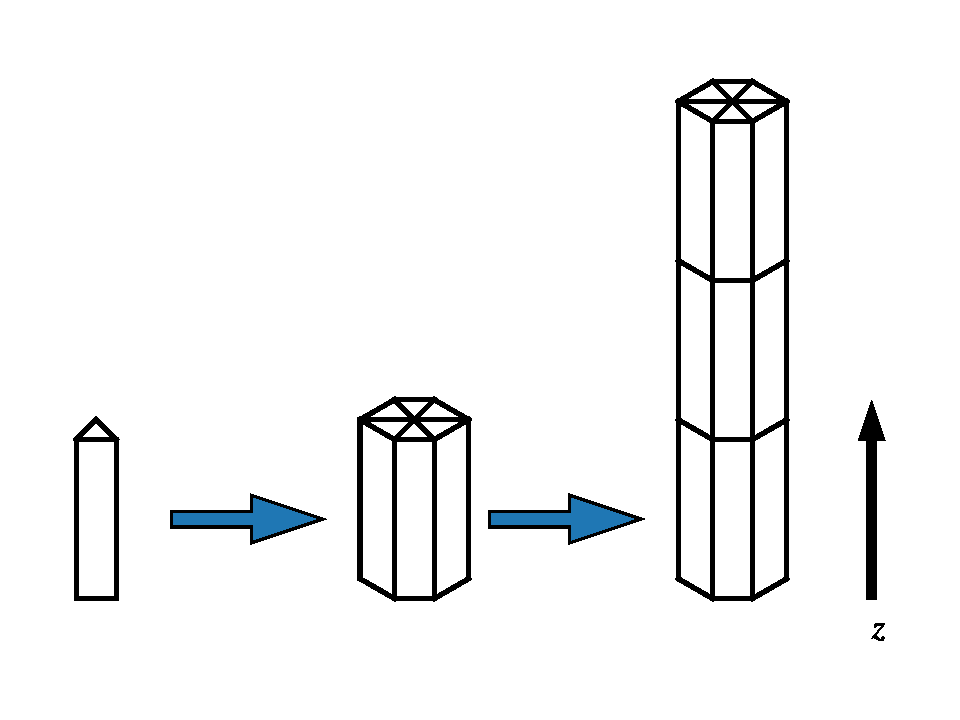
\includegraphics[width=\textwidth]{chunk_description}
        \caption{Progression of Element (left), to Chunk (center), to Channel
          (right).}
        \label{fig:chunk_description}
      \end{figure}
    \end{column}
    \begin{column}{0.5\textwidth}
      \begin{figure}
        \centering
        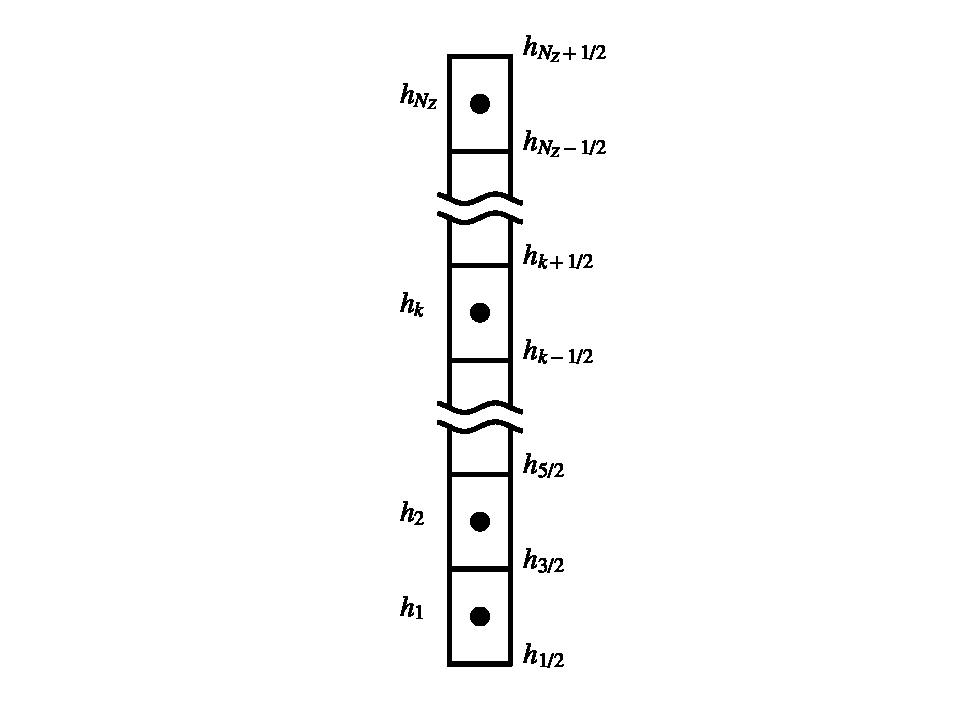
\includegraphics[width=0.35\textwidth]{axial_model}
        %\caption{One-Dimensional Axial Heat Convection Model Description.}
        \label{fig:axial_model}
      \end{figure}
    \end{column}
  \end{columns}
\end{frame}

\begin{frame}{Channel Enthalpy}
  Steady-state coolant enthalpy within the channel is given by an energy
  balance.
  \begin{equation}
    \label{eq:continuous_heat_balance}
    h_i(z) = h_{in} + \frac{1}{\mdot_i} \int_0^z q'_i(z') \; dz'
  \end{equation}
  $h_{in}$ is given by a state relationship from a user-input $T_{inlet}$.
  \begin{equation}
    h_{in} = h(T_{inlet})
  \end{equation}
  Discretize the integral to calculate the enthalpy at the upper node of the
  chunk.
  \begin{equation}
    h_{i,k+1/2} = h_{in} + \frac{1}{\mdot_i} \sum_{k=1}^{N_z} q_{i,k}
  \end{equation}
  Use a first-order approximation to estimate the chunk-average enthalpy.
  \begin{equation}
    h_{i,k} = \half (h_{i,k-1/2}+h_{i,k+1/2})
  \end{equation}
  $T_{\infty,i,k}$ is then given by a state relationship \cite{sodiumProp}.
  \begin{equation}
    T_{\infty,i,k} = T(h_{i,k})
  \end{equation}
\end{frame}

\begin{frame}{Radial Conduction Geometric Model}
  \begin{figure}
    \centering
    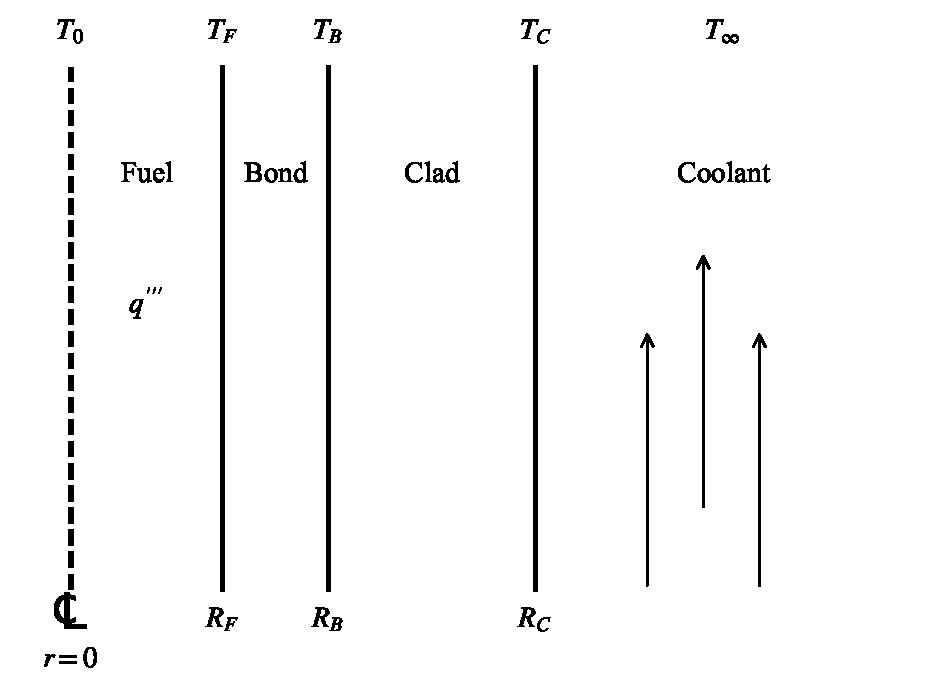
\includegraphics[width=0.7\textwidth]{radial_model}
    \caption{Geometry Description of Radial Heat Conduction Model (not to
      scale).}
    \label{fig:radial_model}
  \end{figure}
\end{frame}

\begin{frame}{Radial Assumptions}
  \begin{itemize}
    \item Axial conduction is negligible within solid materials.
    \item Constant volumetric heat conduction rate within the fuel.
    \item Good thermal contact between materials.
  \end{itemize}
\end{frame}

\begin{frame}{Clad Surface Temperature -- Subbotin-Ushakov}
  Using Newton's Law of Cooling.
  \begin{align}
    q''_{clad} &= H_c (T_C - T_{\infty}) \\
    q''_{clad} &+ q'''_{i,k} \frac{R_F^2}{2 R_C}
  \end{align}
  $H_c$ is given by the Subbotin-Ushakov correlation \cite{subbotinUshakov}
  which relates the Nusselt and P\'eclet numbers for ${1 < Pe < 4,000}$ and 
  ${ 1.2 \le S/D \le 2.0 }$.
  \begin{align}
    Pe &= Re \, Pr \\
    \label{eq:subbotinUshakov}
    Nu &= 7.55 \frac{S}{D} - 20 \left(\frac{S}{D}\right)^{-13} + 
      \frac{3.67}{90\left(\frac{S}{D}\right)^{2}}
      Pe^{\left(0.56 + 0.19 \frac{S}{D}\right)}
  \end{align}
  Then the clad surface temperature, $T_C$ follows.
  \begin{align}
    H_c &= \frac{N\!u \, k}{D_e} \\
    T_C &= \frac{q''_{clad}}{H_c} + T_{\infty}
  \end{align}
\end{frame}

\begin{frame}{Rod Surface Temperatures}
  Once the clad surface temperature is known, subsequent surface temperatures
  are given by radial heat conduction.
  \begin{align}
    \label{eq:tc_forward}
    T_C &= q'''_{i,k} \frac{R_F^2}{2\,R_c\,H_c} + T_{\infty} \\
    \label{eq:tb_forward}
    T_B &= T_C + \frac{q'''_{i,k}}{2 k_C} R_F^2
      \ln\left(\frac{R_C}{R_B}\right) \\
    \label{eq:tf_forward}
    T_F &= T_B + \frac{q'''_{i,k}}{2 k_B} R_F^2 
      \ln\left(\frac{R_B}{R_F}\right) \\
  \end{align}
\end{frame}

\begin{frame}{Fuel Centerline Temperature}
  Define a conductivity integral.
  \begin{equation}
    \label{eq:conductivity_integral}
    K_F(T) = \int_0^T k_F(T') \; dT'
  \end{equation}
  The value of the conductivity integral is given by the heat conduction
  equation.
  \begin{equation}
    \label{eq:tcl_conductivity_integral}
    K_F(T_0) = K_F(T_F) + \frac{q'''_{i,k}}{4} R_F^2
  \end{equation}
  Then, a bisection method search is used to calculate $T_0$ given a functional
  form of $K_F(T)$.
\end{frame}

\begin{frame}{Average Material Temperatures}
  Average temperatures in the clad and bond are calculated analytically.
  \begin{align}
    \label{eq:tb_bar}
    \overline{T_B} &= T_F - \frac{q'''_{i,k}}{4 k_B} \, R_F^2 \, \left(
      \frac{R_F^2 - R_B^2 + 2\,R_B^2 \ln\left(\frac{R_B}{R_F}\right)}
      {R_B^2-R_F^2}\right) \\
    \label{eq:tc_bar}
    \overline{T_C} &= T_B - \frac{q'''}{4 k_C} R_F^2 \left(
      \frac{2 \, R_C^2 \ln\left(\frac{R_C}{R_B}\right)}
      {R_C^2 - R_B^2}  - 1\right)
  \end{align}
\end{frame}

\begin{frame}{Average Fuel Temperature}
  To calculate an average fuel temperature, an effective fuel thermal
  conductivity is calculated.
  \begin{equation}
    \label{eq:kfuel_constant}
    \overline{k_F} = \frac{q'''_{i,k} \, R_F^2}{4(T_0-T_F)}
  \end{equation}
  Fuel thermal conductivity is assumed constant at $\overline{k_F}$ and an
  analytic value is calculated for the average fuel temperature.
  \begin{equation}
    \label{eq:tf_bar}
    \overline{T_F} = T_0 - \frac{q'''_{i,k}}{8 \overline{k_F}} R_F^2
  \end{equation}
  $\overline{T_F}$ is used to calculate fuel cross-sections. Due to
  self-shielding in the fuel, an effective fuel temperature would weight the
  surface temperature more.
\end{frame}

\begin{frame}{Radial Temperatures for Typical Fuel Rod}
  \begin{figure}
    \centering
    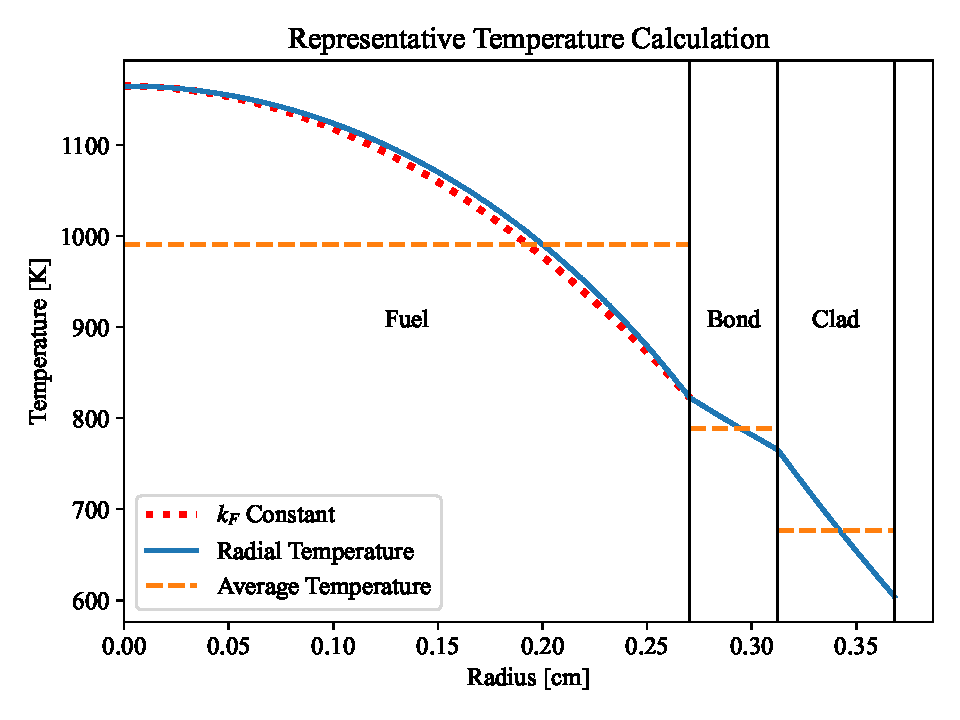
\includegraphics[width=0.7\textwidth]{radial_temp_plot}
    %\caption{Radial Temperatures for Typical Fuel Rod.}
    \label{fig:radial_temp_plot}
  \end{figure}
\end{frame}

\begin{frame}{Axial Temperatures for Typical Fuel Channel}
  \begin{columns}
    \begin{column}{0.5\textwidth}
      \begin{figure}
        \centering
        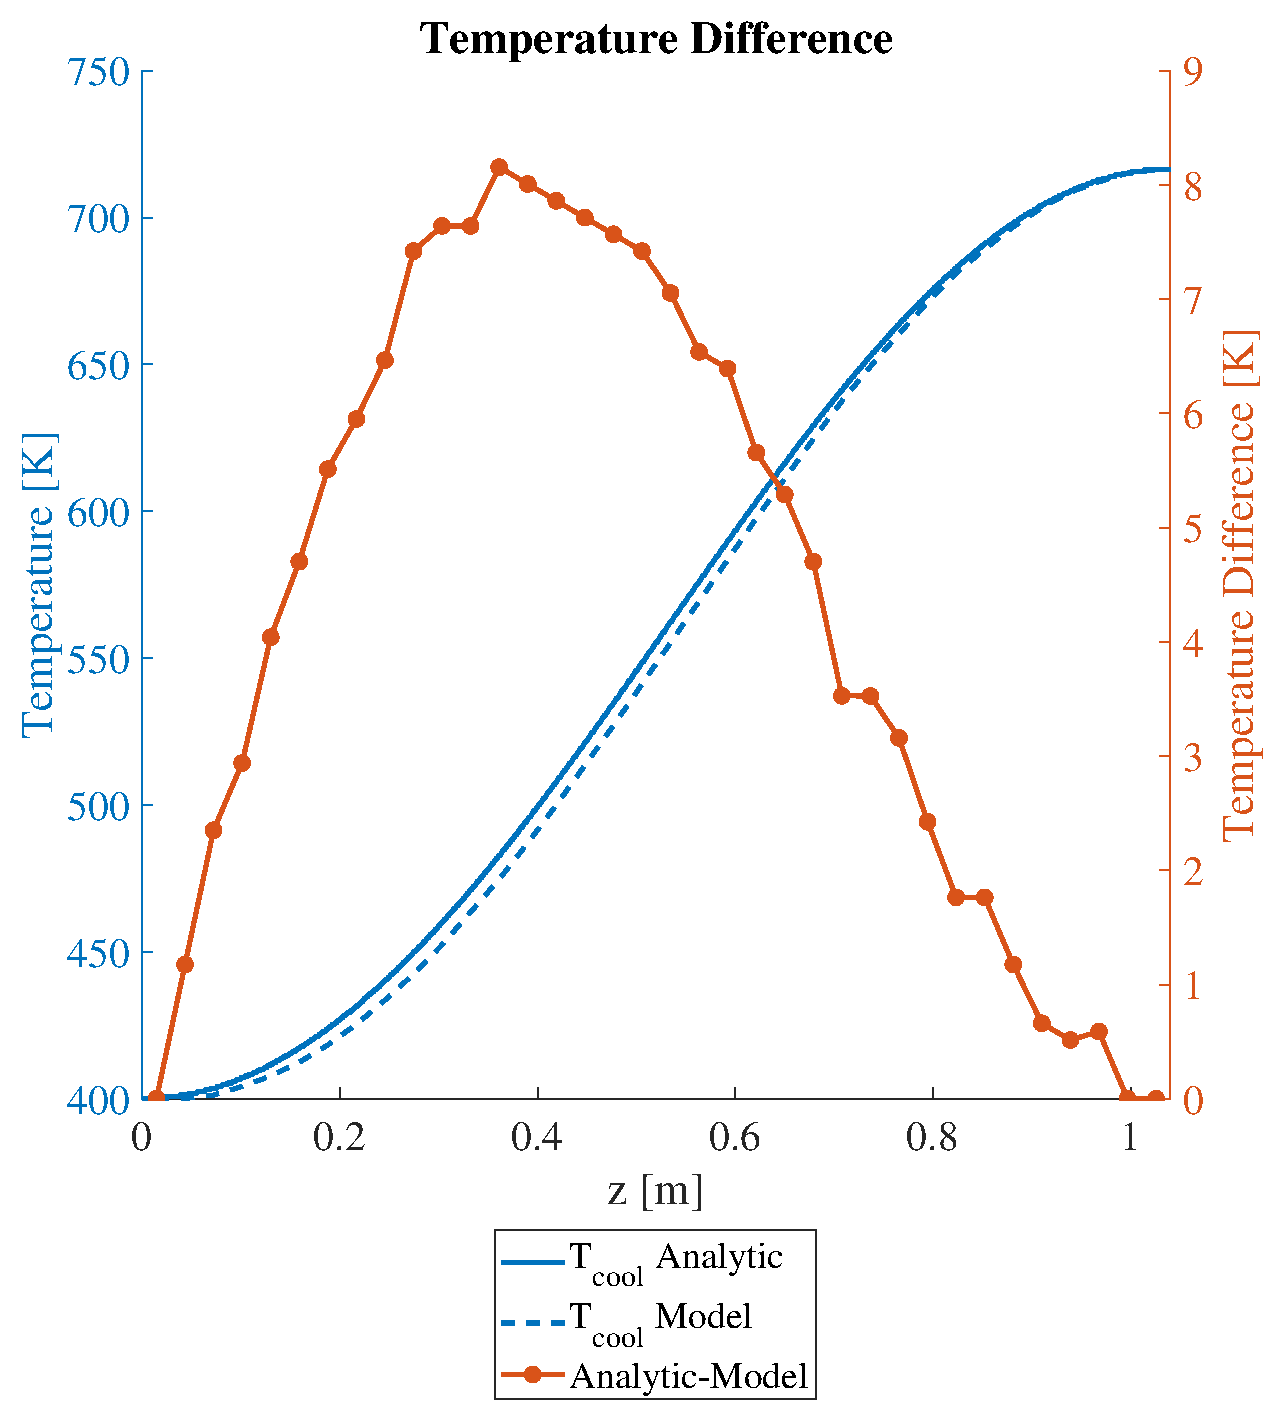
\includegraphics[width=\textwidth]{axial_difference_plot}
        %\caption{Difference Between Analytic and Modeled Axial Temperatures for 36
        %  Axial Levels.}
        \label{fig:axial_difference_plot}
      \end{figure}
    \end{column}
    \begin{column}{0.5\textwidth}
      \begin{figure}
        \centering
        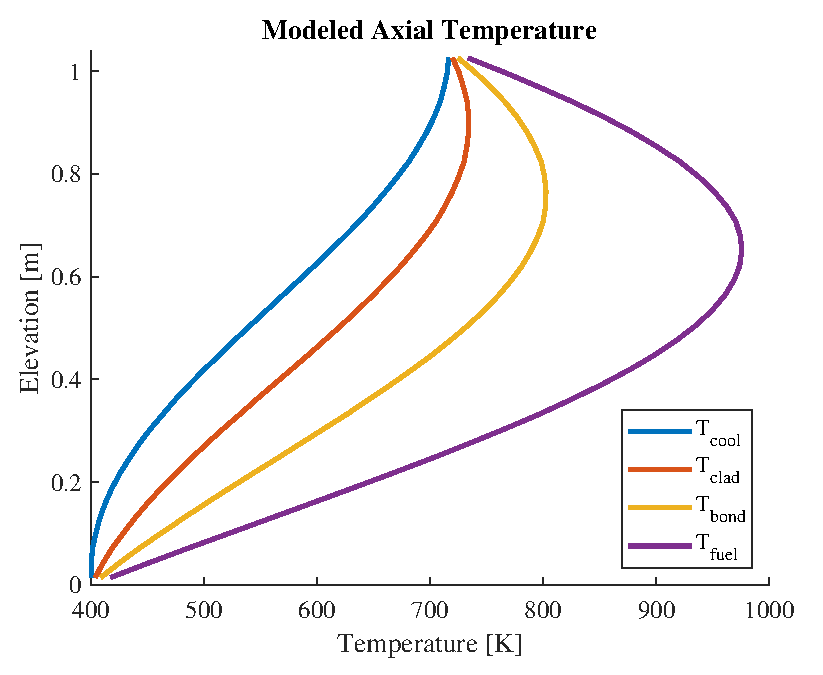
\includegraphics[width=\textwidth]{axial_temp_plot}
        %\caption{Average Axial Temperatures for Model Reactor Conditions.}
        \label{fig:axial_temp_plot}
      \end{figure}
    \end{column}
  \end{columns}
\end{frame}

\begin{frame}{Cross-section Treatment}
  \begin{itemize}
    \item Coolant. 
      \begin{itemize}
        \item Number density and microscopic cross-sections are functionalized 
          and updated based on $T_{\infty,i,k}$.
        \item Linear interpolation for cross sections.
      \end{itemize}
    \item Clad. 
      \begin{itemize}
        \item Macroscopic cross-section updated based on $\overline{T_{C,i,k}}$.
        \item Linear interpolation.
      \end{itemize}
    \item Bond.
      \begin{itemize}
        \item Assumed to have the same macroscopic cross-section as coolant.
        \item Represents a small volume.
        \item Consistent with homogenization approximation.
      \end{itemize}
    \item Fuel.
      \begin{itemize}
        \item Macroscopic cross-section update based on $\overline{T_{F,i,k}}$.
        \item Square-root interpolation due to Doppler effect.
      \end{itemize}
  \end{itemize}
\end{frame}

